%+----------------------------------------------------------------------------+
%| SLIDES: PostDoc interview presentation
%| Duration: 20 minutes
%| Contents: 7 slides
%|					 (extimated duration 3 minutes per slide )
%| Author: Antonio miti
%| Place: Brescia, January 2023
%+----------------------------------------------------------------------------+



%- HandOut Flag -----------------------------------------------------------------------------------------
\newif\ifHandout
	\Handouttrue  %uncomment for the printable version


%- D0cum3nt ----------------------------------------------------------------------------------------------
\ifHandout
	\documentclass[handout,10pt]{beamer}   
	 \setbeameroption{show notes} %print notes   
\else
	\documentclass[10pt]{beamer}
\fi

	
%- Packages ----------------------------------------------------------------------------------------------
\usepackage{./custom-style}
\usepackage{./math}
\usepackage{textpos,eso-pic}
\usepackage{fontawesome}
\usepackage{stmaryrd}


%--Beamer Style-----------------------------------------------------------------------------------------------
\usetheme{toninus}

%- Macros -------------------------------------------------------------------------------------------
\providecommand{\vHam}{\mathscr{v}}

\newcommand{\extrarule}{
		{
			\color{UniGreen}
			\par\hspace*{-\dimexpr0.5\paperwidth-0.5\textwidth}\rule[0.5\baselineskip]{\paperwidth}{0.4pt}
			\vspace{-2em}
		}
}

\renewcommand{\checkpoint}[0]{
	\setcounter{tocdepth}{2}
	\addtocounter{framenumber}{-1}
 	\begin{frame}[t]{Outline}
			\tableofcontents[currentsection,currentsubsection]
	\end{frame}
}


%- TEMP -----------------------------------------------------------------------------
\newtcolorbox[auto counter,number within=section]{probox}[2][]{%
	fonttitle= \footnotesize \bfseries,
	title=#2,
	fontupper=\footnotesize,%\sffamily,
	colback=white,
	colbacktitle=white,
	coltitle=orange!70!black,
	colframe=orange!70!black,
	%boxrule=1pt,
	titlerule=0pt,
	toptitle=-0.2em,bottomtitle=-0.2em, %title spacing	
	colback=white,
	leftupper=-3mm,rightupper=0mm,top=0mm,bottom=0mm, 
	#1,
}

\renewcommand{\action}{\curvearrowright}


%- T1tle P4g3 -------------------------------------------------------------------------------------------
\title{\LARGE Research overview \vspace{-.5em}} 
%\subtitle{}
\author[AMM]{\large \href{https://dmf.unicatt.it/miti/}{Antonio Michele Miti}}
\institute[UCSC]{
	\vspace{1em}
	\\
	Dipartimento di Matematica e Fisica,\\
	Universit\'a Cattolica del Sacro Cuore, 
	Brescia, Italy 
	\\
	\href{https://www.mpim-bonn.mpg.de/}{
\includegraphics[width=5cm]{./Logos/Ucsc_logo}}
	\vspace{1em}
}
\date[Mpim_22] % (optional, should be abbreviation of conference name)
{	
	{\vskip 1ex}
	Unimib Interview, February 8, 2023
}


%---------------------------------------------------------------------------------------------------------------------------------------------------
%- D0cum3nt ----------------------------------------------------------------------------------------------------------------------------------
\begin{document}
%------------------------------------------------------------------------------------------------

%-------------------------------------------------------------------------------------------------------------------------------------------------
\maketitle
%-------------------------------------------------------------------------------------------------------------------------------------------------


%-------------------------------------------------------------------------------------------------------------------------------------------------
\begin{frame}[fragile]{Project title}
\tikzstyle{every picture}+=[remember picture]
	\begin{columns}
    	\begin{column}{.45\textwidth}
    		\onslide<2->{
			\tikz[baseline]{
		            \node[draw=orange!40,anchor=base,text width=5cm] (s1)
		            {Generalization of symplectic geometry in which the symplectic form is generalized from a closed $2$-form to a closed $n+1$-form.};
			}
		}
	\end{column}
    	\begin{column}{.45\textwidth}
    		\onslide<3->{
			 \tikz[baseline]{
		            \node[draw=blue!40,anchor=base, text width=5cm] (s2)
		            {Higher analogue of moment maps in the context of group actions preserving the multisymplectic form.};
			}
		}
	\end{column}
	\end{columns}

	\vfill

	\begin{center}
		\large
		 \tikz[baseline]{
		            \node[fill=orange!20,anchor=base] (t1)
		            {Multisymplectic manifolds};
			}
		 , 
		 \tikz[baseline]{
		            \node[fill=blue!20,anchor=base] (t2)
		            {homotopy comomentum maps};
		        } 
		, 
		\\
		 \tikz[baseline]{
	            \node[fill=green!20,anchor=base] (t3)
	            {$L_\infty$-algebras};
		}
		, and
		 \tikz[baseline]{
	            \node[fill=red!20,anchor=base] (t4)
	            {applications};
		}		
	\end{center}

	\vfill

	\begin{columns}
    	\begin{column}{.45\textwidth}
    		\onslide<4->{
	 		 \tikz[baseline]{
	            \node[draw=green!40,anchor=base,text width=5cm] (s3)
	            {Higher generalization of Lie algebras where the Jacobi identity is allowed only "up to homotopies".};
	         }
		}		   	
		\end{column}
    	\begin{column}{.45\textwidth}
    		\onslide<5->{
				\tikz[baseline]{
	            \node[draw=red!40,anchor=base,text width=5cm] (s4)
	            {Classical field theories, \\prequantization, \\geometric approach to Pdes, \\variational calculus, \\integrators ...};
	           }	
			}
		\end{column}
	\end{columns}

	\begin{tikzpicture}[overlay]
        \path[->,draw=orange!40]<2-> (s1) edge [bend right] (t1);
        \path[->,draw=blue!40]<3-> (s2) edge [bend left] (t2);
        \path[->,draw=green!40]<4-> (s3) edge [bend left] (t3);
        \path[->,draw=red!40]<5-> (s4) edge [bend right] (t4);
	\end{tikzpicture}


\end{frame}
\note[itemize]{
	\item Provide a vague idea of the words that make up the title.
	\item
	\item Conventions:
	\\- $M$ and $G$ are connected,
	\\- actions $\theta:G \curvearrowright M$ are always smooth
	\\- $\xi,\eta\in\mathfrak{g}$,
	\\- for $\mu\in\Omega^*(M,\mathfrak{g}^*)$ and $\xi\in\mathfrak{g}$, write
			\[
				\mu_\xi := \langle\mu,\xi\rangle \;{\color{black!50}\in\Omega^*(M)}
			\]
			for the ``$\xi$th component'' of $\mu$.
}
%-------------------------------------------------------------------------------------------------------------------------------------------------


%-------------------------------------------------------------------------------------------------------------------------------------------------
\section{Research Statement}
%-------------------------------------------------------------------------------------------------------------------------------------------------
%-------------------------------------------------------------------------------------------------------------------------------------------------
\subsection{Framework}
\checkpoint
%-------------------------------------------------------------------------------------------------------------------------------------------------

%-------------------------------------------------------------------------------------------------------------------------------------------------
\begin{frame}[t, fragile]{Research Framework:  \textbf{multisymplectic geometry}} %Fragile -->workaround tikzcd
	\begin{center}
		$-$ \emph{multisymplectic means \textbf{going higher} in the degree of $\omega$} $-$
	\end{center}
	\pause
	\begin{defblock}[$n$-plectic manifold ~\emph{(Cantrijn, Ibort, De Le\'on)} \cite{Cantrun2017}]
		\includestandalone[width=0.95\textwidth]{./Pictures/Figure_multisym}	
	\end{defblock}
	%
	\vfill
	%
	%
	\pause
	\begin{block}{Examples:}
		\begin{itemize}
			\item[$\bullet$] 1-plectic $=$ symplectic
			\item[$\bullet$] Any oriented $(n+1)$-dimensional manifold is $n$-plectic w.r.t. the volume form.
			\item[$\bullet$] The multicotangent bundle $\Lambda^n T^\ast Q$ is naturally $n$-plectic.
		\end{itemize}
	\end{block}			 
%
	\pause
	\begin{block}{Historical motivation}
		Mechanics: geometrical foundations of \textit{(first-order)} field theories.
		\begin{itemize}
		 \item[•] Kijowski, W. Tulczyjew \cite{Kijowski1979}; %(1979)
		 \item[•] Cariñena, Crampin, Ibort \cite{Carinena1991b};% (1991)
		 \item[•] Gotay, Isenberg, Marsden, Montgomery \cite{Gimmsy1};%(1998)
		 \\ $\cdots$
		\end{itemize}
	\end{block}
\end{frame}
%-------------------------------------------------------------------------------------------------------------------------------------------------


%-------------------------------------------------------------------------------------------------------------------------------------------------
\begin{frame}{Observables in \textbf{multisymplectic geometry}}
	%
	\begin{defblock}[Hamiltonian $(n-1)$-forms]
		\begin{displaymath}
			\Omega^{n-1}_{ham}(M,\omega) 	:=
			\biggr\{ \sigma \in  \Omega^{n-1}(M) \; \biggr\vert \; 
				\exists \vHam_\sigma \in \mathfrak{X}(M) ~:~ 
				\tikz[baseline,remember picture]{\node[rounded corners,
                        fill=orange!5,draw=orange!30,anchor=base]            
            			(target) {$d \sigma = -\iota_{\vHam_\sigma} \omega$ };
            	}				
				~\biggr\} 
			\end{displaymath}
	\end{defblock}
	%
	\onslide<2>{
		\tikz[overlay,remember picture]
		{
			\node[rounded corners,
                 fill=orange!5,draw=orange!30,anchor=base]
            	 (base) at ($(current page.north east)-(2,1)$) [rotate=-0,text width=3.5cm,align=center] {\footnotesize{\textcolor{red}{Hamilton-DeDonder-Weyl \\equation}}};
		}	
		\begin{tikzpicture}[overlay,remember picture]
		    	\path[->] (base.south east) edge[bend left,red](target.east);
	    \end{tikzpicture}
	}
	%
	\vspace{-1em}
	\pause
	\begin{columns}[T]
		\setlength{\belowdisplayskip}{5pt}
		\begin{column}{.50\linewidth}
			%
			\centering \it
			$-$ symplectic case $-$
			\onslide<3->{
			\begin{thmblock}[Observables Poisson algebra]
				$C^\infty(M,\omega)$ endowed with
				\vspace{-.5em}
				\begin{displaymath}
					\lbrace \sigma_1, \sigma_2 \rbrace =			
					~ - \iota_{\vHam_1}\iota_{\vHam_2} \omega 
					~= \mathcal{L}_{\vHam_1} \sigma_2
				\end{displaymath}			
				forms a Poisson algebra.
			\end{thmblock}
			}
			%
			\onslide<4->{
			\vspace{1em}
			\begin{itemize}
				\item[\cmark] Skew-symmetric;
				\item[\cmark] multiplication of observables;
				\item[\cmark] Leibniz Rule;
				\item[\cmark] Jacobi equation;
			\end{itemize}		
			}		
		\end{column}	
		%
		\onslide<1->{\vrule{}}
		%
		\begin{column}{.50\linewidth}
			\centering \it
			$-$ $n$-plectic case $-$
			\onslide<5->{			
			\begin{thmblock}[Observables $L_\infty$-algebra]
				$\Omega^{n-1}_{ham}(M,\omega)$ endowed with
				\vspace{-.5em}
				\begin{displaymath}
					\lbrace \sigma_1, \sigma_2 \rbrace =			
					~ - \iota_{\vHam_1}\iota_{\vHam_2} \omega 
				\end{displaymath}			
				can be extended to a \\ $L_\infty-algebra$.
			\end{thmblock}
			}
			%
			\onslide<6->{
			\begin{itemize}
				\item[\cmark] Skew-symmetric;
				\item[\xmark] multiplication of observables;
				\item[\xmark] Jacobi equation;
				%\\ \hspace*{4.25em} full-fledged Jacobi equation;
				\item[\smark] Jacobi equation \emph{up to homotopies}.
			\end{itemize}			
			}
		\end{column}	
	\end{columns}
\end{frame}
%-------------------------------------------------------------------------------------------------------------------------------------------------



%-------------------------------------------------------------------------------------------------------------------------------------------------
\begin{frame}[t]{Symmetries in \textbf{multisymplectic geometry}}
	Consider a Lie algebra action $v:\mathfrak{g} \to \mathfrak{X}(M)$  preserving the $n$-plectic form $\omega$,
	\vfill

	\vspace{-1em}
	\begin{columns}[T]
		\setlength{\belowdisplayskip}{5pt}
		\begin{column}{.50\linewidth}
			%
			\centering \it
			\onslide<2->{
				$-$ symplectic case $-$
				\begin{defblock}[Comoment map pertaining to $v$]
					Lie algebra morphism
					$$ f: \mathfrak{g} \to C^\infty(M) $$
					such that
					$$ d~f (x) = -\iota_{v_x} \omega \qquad \forall x \in \mathfrak{g}~.$$
				\end{defblock}
			}
		\end{column}	
		%
		\onslide<2->{\vrule{}}
		%
		\begin{column}{.50\linewidth}
			\centering \it
			\onslide<3->{			
				$-$ $n$-plectic case $-$
				\begin{defblock}[Homotopy comoment map \tiny (HCMM)]
					$L_\infty$-morphism 
					$$ (f_k) : \mathfrak{g} \to L_\infty (M,\omega)$$
					such that
					$$ d~f_1(x) = -\iota_{v_x} \omega \qquad \forall x \in \mathfrak{g}~.$$
				\end{defblock}	
			}
		\end{column}	
	\end{columns}	
	%
	\pause
	\vfill
	\centering 
	\onslide<4->{\textbf{-- Conserved quantities --}}
	%
	\vspace{-.5em}
	\begin{columns}[T]
		\setlength{\belowdisplayskip}{5pt}
		\begin{column}{.50\linewidth}
			%
			\centering \it
			\onslide<4->{
			\begin{propblock}[Noether Theorem]
				\small Fixed $H\in C^\infty_{\text{Ham}}(M)$ ($\mathfrak{g}$-invariant) ,
				$$\mathcal{L}_{v_H} f(x) = 0 \qquad \forall x \in \mathfrak{g}$$
			\end{propblock}
			}
		\end{column}	
		%
		\onslide<5->{\vrule{}}
		%
		\begin{column}{.50\linewidth}
			\centering \it
			\onslide<5->{			
			\begin{propblock}[RWZ16 Theorem]
				\small Fixed $H\in \Omega^{n-1}_{\text{Ham}}(M)$ ($\mathfrak{g}$-invariant),
				$$\mathcal{L}_{v_H} f_k(p) \in B^k(M) \qquad \forall p \in Z_k(\mathfrak{g})$$			
			\end{propblock}
			}
		\end{column}	
	\end{columns}		
\end{frame}
%-------------------------------------------------------------------------------------------------------------------------------------------------


%-------------------------------------------------------------------------------------------------------------------------------------------------
\subsection{Results}
\checkpoint
%-------------------------------------------------------------------------------------------------------------------------------------------------

%-------------------------------------------------------------------------------------------------------------------------------------------------
\subsubsection{JW Mauro}
%-------------------------------------------------------------------------------------------------------------------------------------------------
	\begin{frame}[t]{Applications to hydrodynamics and knot theory \small(J.w. M.Spera)}

		\begin{columns}
			\begin{column}[T]{0.2\textwidth}
				\centering
					\fbox{
\includegraphics[width=.9\textwidth]{./Pictures/cover-JAMS}}
			\end{column}		
			\begin{column}[T]{0.8\textwidth}
				\vspace{-.25em}
				\begin{center}
					\textbf{On some (multi)symplectic aspects of link invariants}, \\ 
					\emph{AMM, Mauro Spera}, \href{https://arXiv.org/abs/1805.01696}{arxiv:1805.01696};\\
					(Appeared in \emph{Journal of the Australian Mathematical Society})	
				\end{center}			
			\end{column}		
		\end{columns}	
		\extrarule
	
		\vfill
		\begin{columns}
			\begin{column}{.3\linewidth}
				$G~=~SDiff_0(\mathbb{R}^3)$
				\\
				(volume-preserving diffeomorphisms)
			\end{column}	
			\pause
			\begin{column}{.7\linewidth}
				\begin{itemize}
					\item Configuration space of an \emph{ideal fluid},
					\item (Determining) ambient isotopies of knotted links (interpreted as singular vortices)
				\end{itemize}
			\end{column}
		\end{columns}
		%
		\pause
		\begin{columns}
			\begin{column}{.45\linewidth}
			  	\begin{displaymath}
			  		\begin{split}
			  		&\mathfrak{g}:= sdiff_0(\mathbb{R}^3) = \\
			  		&\left\lbrace  X \in \mathfrak{X}(\mathbb{R}^3) ~\left\vert~ 
			  		\substack{ div X = 0, \\ \textrm{\emph{ rapidly vanishing at }}\infty} \right\rbrace \right.
			  		\end{split}
			  	\end{displaymath}
			\end{column}	
			\begin{column}{.55\linewidth}
				\begin{itemize}
					\item Fluid velocities
					\item Subalgebra of the  $\infty$-dim. "Lie algebra" of a $\infty$-dim "Lie group" $G$.
				\end{itemize}
			\end{column}
		\end{columns}
		\pause

		\vfill
		\tcbset{colback=white,
			colbacktitle=white,
			colframe=blue!70!black,
			boxrule=1pt,
			colupper=blue!70!black,
			arc=15pt,
			}
		\begin{tcolorbox}[sidebyside,righthand width=.75\linewidth]
			Thm: \cite{Miti2018}
			\tcblower
			%
			\centering
			\vspace{-.5em}
			Multisymplectic Lie algebra action $\mathfrak{g}= sdiff_0 \hookrightarrow  \mathfrak{X}(\mathbb{R}^3)$, \\
			w.r.t $(\mathbb{R}^3,\nu = dx\wedge dy\wedge dz)$ 2-plectic mfd, \\
			\alert{admits an HCMM}.
			\vspace{-.5em}
		\end{tcolorbox}	

		%
		\vfill
		\begin{itemize}[<+->]%[<alert@+>]
			\item[\CheckedBox]  Hydrodynamics interpretation: Rasetti-Regge currents as "momenta".
			% is exhibited upon resorting to the Euler equation for perfect fluids.
			\item[\CheckedBox]  Knot theory: reinterpretation of the (Massey) higher order linking numbers in terms of conserved quantities.
			%\item[\CheckedBox]  Semiclassical interpretation of the HOMFLYPT polynomial.
		\end{itemize}
		%	
	\end{frame}
%---------------------------------------------------------------------------------------------------------------------------------------------------





%-------------------------------------------------------------------------------------------------------------------------------------------------
\subsubsection{JW Leonid}
%-------------------------------------------------------------------------------------------------------------------------------------------------
	\begin{frame}[t]{Compact multisymp. actions on spheres \small (J.w. L.Ryvkin)}
		%
		\begin{columns}[T]
			\begin{column}{0.2\textwidth}
				\centering
					\fbox{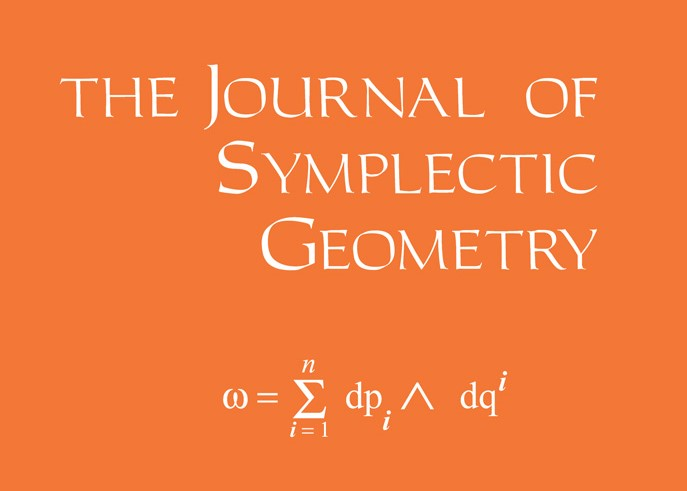
\includegraphics[width=.9\textwidth]{./Pictures/cover-JSG}}
			\end{column}		
			\begin{column}{0.8\textwidth}
				\begin{center}
					\textbf{Multisymplectic actions of compact Lie groups on spheres}, \\
					\emph{AMM, Leonid Ryvkin}, \href{https://arxiv.org/abs/1906.08790}{arXiv:1906.08790};\\
					(Appeared in \emph{Journal of Symplectic Geometry})	
				\end{center}		
			\end{column}		
		\end{columns}				
		\extrarule
		\pause
		\vspace{1em}
		%
		
		Consider the multisymplectic manifold $(S^n,\omega)$ given by the $n$-dimensional sphere together with the standard volume.
		
		\tcbset{colback=white,
			colbacktitle=white,
			colframe=blue!70!black,
			boxrule=1pt,
			colupper=blue!70!black,
			arc=15pt,
			}
		\begin{tcolorbox}[sidebyside,righthand width=.75\linewidth]
			Thm: \cite{Miti2019}
			\tcblower
			%
			\centering
			\vspace{-.5em}
			Let $\vartheta:G\times S^n \to S^n$ be an effective, compact, multisymplectic action,
				\begin{center}
					\alert{$\vartheta$ admits HCMM $~\Leftrightarrow~$ $n$ is even or $\vartheta$ is not transitive}.
				\end{center}
			\vspace{-.5em}
		\end{tcolorbox}	
		%
		\vfill
		\pause
	%
	\begin{itemize}
		\item[\CheckedBox]  Complete classification of Hamiltonian actions on spheres (multisymplectic w.r.t. the canonical volume form);
		\item[\CheckedBox]  	Explicit construction for 
	$SO(n)~\circlearrowleft~S^{n}$ and
	$G_2~\circlearrowleft~(S^6,\phi)$;
		\item[\CheckedBox]   Explicit expression for the first 2 components of HCMM for 
			$SO(n+1)~\circlearrowleft~S^{n}$.
		 %(Going higher can be set up as a computational problem. We sketched a prototype code in python.)
	\end{itemize}	
		
\end{frame}
%---------------------------------------------------------------------------------------------------------------------------------------------------




%-------------------------------------------------------------------------------------------------------------------------------------------------
\subsubsection{JW Marco}
%-------------------------------------------------------------------------------------------------------------------------------------------------
	\begin{frame}[t]{Multisymp. observables and Vinogradov algebroids \small (Jw. M.Zambon)}
		\begin{columns}[T]
			\begin{column}{0.2\textwidth}
				\centering
					\fbox{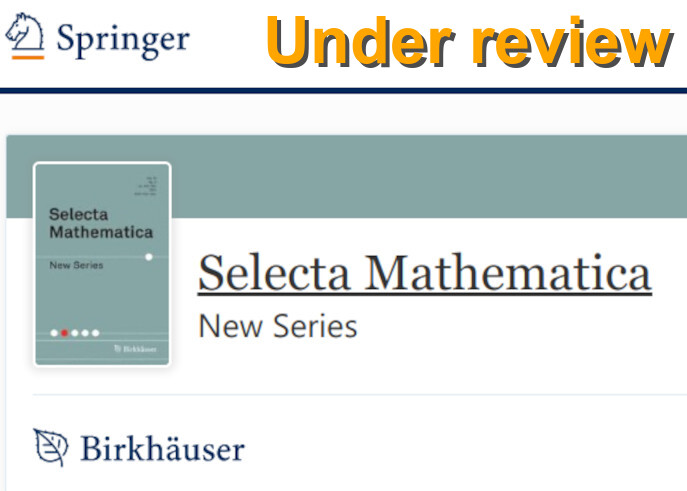
\includegraphics[width=.9\textwidth]{./Pictures/cover-Selecta-honest}}
			\end{column}		
			\begin{column}{0.8\textwidth}
				%
				\centering
				\textbf{Observables of multisymplectic manifolds\\ and higher Courant algebroids},
				\\
				\emph{AMM, Marco Zambon}; \href{https://arxiv.org/abs/2209.05836}{arxiv:2209.05836};\\
				(Submitted to \emph{Selecta Mathematica}.)	
			\end{column}		
		\end{columns}
		\extrarule
		\vspace{1em}
		
		\includestandalone[width=.95\textwidth]{../Pictures/Frame_BigDiagram_k-plectic}
		
		\vfill
	\tcbset{colback=white,
		colbacktitle=white,
		colframe=blue!70!black,
		boxrule=1pt,
		colupper=blue!70!black,
		arc=15pt,
		}
	\onslide<5->{
	\begin{tcolorbox}[sidebyside,righthand width=.75\linewidth]
		Thm: \cite{Miti2021}
		\tcblower
		\vspace{-.5em}
		\begin{itemize}
			\item[-]<.-|alert@.>
				There is an embedding of $L_\infty$-algebras  $L_\infty(M,\omega)\hookrightarrow L_{\infty}(\mathbb{T}M,\omega)$.
			\item[-]<8-|alert@+> The central square commutes. 		\vspace{-.5em}
		\end{itemize}
	\end{tcolorbox}	}
		
		
\end{frame}
\note[itemize]{
	\item Compatibility of \emph{Homotopy comomentum maps} w.r.t. gauge-related multisymplectic manifolds.
	\item 	Relationship between the $L_\infty$-algebra of observables and \emph{higher courant algebroids.} 
	\item Given a Symp. mfd. $(M,\omega)$ there is a naturally associated Poisson algebra ...
	\item {... and also a Lie Algebroid}.
	\item A Lie algebroid is a "controlled" $\infty$-dimensional Lie algebra;
	\item Consider a deformed structure $\tilde{\omega}= \omega + d B$ with $B\in C^\infty(M)$;
	\item There is a natural isomorphism in the Lie Alg.oids category,
	\item Considering $\mathfrak{g}\circlearrowleft M$ preserving $\omega$ and $\tilde{\omega}$ ...
	\item The horizontal embedding is  $f \mapsto (v_f,f)$;
	\item Vertical maps are also known as \emph{Gauge transformations}
	\item Higher analogue of the Courant algebroid $\rightsquigarrow$ \emph{Vinogradov algebroid} $\mathbb{T}M =(TM\oplus\bigwedge^{k-1}T^\ast M)$
	\item Vin. alg.oids are $NQ$-manifolds, there's associated $L_\infty$-algebra
	\item Our results can be seen as a tiny step toward  undestanding the analogue of prequantization in the setting of multisymplectic geometry (hence field theory).
}
%-------------------------------------------------------------------------------------------------------------------------------------------------



%-------------------------------------------------------------------------------------------------------------------------------------------------
\subsubsection{JW LeoCas}
%-------------------------------------------------------------------------------------------------------------------------------------------------
	\begin{frame}[t,fragile]{Results}
	%
	\tikzstyle{every picture}+=[remember picture]
	%
		\begin{columns}[T]
			\begin{column}{0.2\textwidth}
				\centering
					\fbox{
\includegraphics[width=.9\textwidth]{./Pictures/cover-PJM-honest}}
			\end{column}		
			\begin{column}{0.8\textwidth}
				\centering
				\textbf{Reduction of $L_\infty$-algebras of observables\\ on multisymplectic manifolds},
				\\
				\emph{Casey Blacker, AMM, Leonid Ryvkin}; \href{https://arxiv.org/abs/2206.03137}{arxiv:2206.03137};\\
				(Submitted to \emph{Pacific Journal of Mathematics}.)	
			\end{column}		
		\end{columns}
		\extrarule
		
		\vfill
		%
		\begin{itemize}
			\item \cite{Blacker2020}: multisymplectic analogue of MWM reduction.
			\item What about the non regular case? \quad \alert{Observables reduction}
		\end{itemize}		
		\vfill
		\pause
		
		\tcbset{colback=white,
			colbacktitle=white,
			colframe=blue!70!black,
			boxrule=1pt,
			colupper=blue!70!black,
			arc=15pt,
		}
		\begin{tcolorbox}[sidebyside,righthand width=.75\linewidth]
			Thm: \cite{Blacker2022}
			\tcblower
			
				Let $\g\curvearrowright M$ be a preserving  $\omega$  ($k$-plectic form) and $N\subset M$.\\[2pt]

		The \emph{reduced observables}  $L_\infty$-algebra is
		\begin{columns}
			\begin{column}{.80\linewidth}
			 	\begin{displaymath}
			 		\Ham_\infty(M,\omega)_N = 
			 		\frac{
			 			\tikz[baseline]{
			 				\node[fill=orange!20, ellipse, anchor=base] (t1) 
			 				{$ \Ham_\infty(M,\omega)_{[N]}$};}
			 		}{
			 			\tikz[baseline]{
			 				\node[fill=blue!20, ellipse,anchor=base] (t2)
			 				{$I_{\Ham_\infty}(N)$};
			 			}
			 		}
			 		~.
			 	\end{displaymath}
			\end{column}
			\begin{column}{.3\linewidth}
								\tikz[baseline]{
		            				\node[draw=orange!40,anchor=base,text width=.95\linewidth] (s1)
		            				{obs. \textbf{reducible}\\ along $N$,};
								}
				\\[4pt]
								\tikz[baseline]{
		            				\node[draw=blue!40,anchor=base,text width=.95\linewidth] (s2)
		            				{obs. \textbf{vanishing}\\ along $N$.};
								}
			\end{column}
		\end{columns}

			
			

			
		\end{tcolorbox}	
		
	\begin{tikzpicture}[overlay]
        \path[->,draw=orange!40]<2-> (s1) edge [bend right] (t1);
        \path[->,draw=blue!40]<3-> (s2) edge [bend left] (t2);
	\end{tikzpicture}
		
\end{frame}
%---------------------------------------------------------------------------------------------------------------------------------------------------






%-------------------------------------------------------------------------------------------------------------------------------------------------
\section{Research Proposal}
\subsection{Ongoing projects}
\checkpoint
%-------------------------------------------------------------------------------------------------------------------------------------------------

%-------------------------------------------------------------------------------------------------------------------------------------------------
\begin{frame}{Observables quantities in multisymplectic geometry}

\end{frame}
\note[itemize]{
	\item  Research Line A

}
%-------------------------------------------------------------------------------------------------------------------------------------------------

%-------------------------------------------------------------------------------------------------------------------------------------------------
\begin{frame}{Observables Algebras in $n$-plectic geometry}
	%
	\alert{There are at least two competing notions of "observables" in multisym. geo. :}
	%
	\vspace{-1em}
	\begin{columns}[T]
		\pause
		\setlength{\belowdisplayskip}{5pt}
		\begin{column}{.50\linewidth}
			%
			\begin{thmblock}[Observables $L_\infty$-algebra]
				$\Omega^{n-1}_{ham}(M,\omega)$ endowed with
				\vspace{-.5em}
				\begin{displaymath}
					\lbrace \sigma_1, \sigma_2 \rbrace =			
					~ - \iota_{\vHam_1}\iota_{\vHam_2} \omega 
				\end{displaymath}			
				can be "completed" to a \\ $L_\infty-algebra$.
			\end{thmblock}
			%
			\pause
			\begin{itemize}
				\item[\cmark] Skew-symmetric;
				\item[\xmark] multiplication of observables;
				\item[\xmark] Jacobi equation;
				%\\ \hspace*{4.25em} full-fledged Jacobi equation;
				\item[\smark] Jacobi equation \emph{up to homotopies}.
			\end{itemize}				
		\end{column}	
		%
		\onslide<1->{\vrule{}}
		%
		\pause
		\begin{column}{.50\linewidth}
			\begin{thmblock}[Observables Leibniz algebra]
				$\Omega^{n-1}_{ham}(M,\omega)$ endowed with
				\vspace{-.5em}
			\begin{displaymath}
				\llbracket \sigma_1, \sigma_2 \rrbracket =
				~ \mathcal{L}_{\vHam_1} \sigma_2
				~.					
			\end{displaymath}		
				can be "completed" to a \\ DG-Leibniz algebra.
			\end{thmblock}	
			%
			\pause
			\begin{itemize}
				\item[\xmark] Skew-symmetric;
				\item[\xmark] multiplication of observables;
				\item[\cmark] Jacobi equation;
				\item[\smark] Skew-symmetric \emph{up to homotopies}.
			\end{itemize}	
		\end{column}	
	\end{columns}
	
	\vfill
	
	\begin{probox}[colbacktitle=yellow!15!white ,colback=yellow!15!white]{ What is the \emph{"correct"} notion of observables?}
		\begin{itemize}
			\item[\cmark] Preliminary results on $2$-plectic prequantization due to Sevestre and Wurzbacher:
			\item[\smark] Does $L_\infty(M,\omega)$ relate with the $L_\infty$-extension of $Leib(M,\omega)$ provided by \cite{Lavau2020} ?
			\item[\smark] Are they two different aspects of a third, more general, algebraic structure (e.g. \emph{weak $L_\infty$-algebras provided by \cite{Dehling2017})}
		\end{itemize}
	\end{probox}		
	
\end{frame}
\note[itemize]{
 \item See \cite[\S 7.2]{Rogers2010} about the comparison of these two algebraic structures.
 \item Notice that the failure of skew-symmetricity is measured by
 \begin{align*}
 	A(\sigma_1,\sigma_2) 
 	=&~
 	 2~\llbracket \sigma_1, \sigma_2\rrbracket +  \llbracket \sigma_2, \sigma_1\rrbracket
 	 \\
 	 =&~ d \circ\langle\sigma_1,\sigma_2\rangle_+
 \end{align*}
 (Compare with the \href{https://en.wikipedia.org/wiki/Courant_bracket\#Dorfman_bracket}{Dorfmann bracket}.)
 
 \item Notice that the antisymmetrization of $\llbracket \cdot, \cdot \rrbracket$ equates $\lbrace \cdot,\cdot \rbrace$ modulo homotopy:
 \begin{align*}
  \llbracket \sigma_1,\sigma_2 \rrbracket  \circ 	\mathcal{A}
  =&~
  \frac{\mathcal{L}_{\vHam_1}\sigma_2 - \mathcal{L}_{\vHam_2}\sigma_1}{2} 
  \\
  =&~ 
  \frac{1}{2}( d (\iota_{\vHam_1}{\sigma_2} - \iota_{\vHam_2}{\sigma_1} )
  +\frac{1}{2}(-\iota_{\vHam_1}\iota_{\vHam_2}\omega + \iota_{\vHam_2}\iota_{\vHam_1}\omega) 
  \\
  =&~
  \lbrace \sigma_1, \sigma_2 \rbrace + d \circ \langle\sigma_1,\sigma_2\rangle_-
  \\
  =&~
  [\sigma_1,\sigma_2]_\omega
 \end{align*}
 where the last bracket is given by the Vinogradov algebroid Binary bracket.
 \item GOALS: \textit{
Explicitly construct a morphism, inside the category of Lie infinity algebras, between $L_\infty(M,\omega)$ and the \emph{$L_\infty$-extension} of $Leib(M,\omega)$.
Discuss the functoriality of the two $L_\infty$-algebras considered above and the naturality of the sought morphism connecting each other.
Construct a so-called \emph{weak $L_\infty$-algebra} structure encoding both $L_\infty(M,\omega)$ and $Leib(M,\omega)$.
Compare the latter construction to other approaches to multisymplectic observables like \cite{Delgado2018b} and \cite{Herman2018a}.
}
}
%-------------------------------------------------------------------------------------------------------------------------------------------------


%-------------------------------------------------------------------------------------------------------------------------------------------------
\begin{frame}{Open questions on covariant observables (Preliminary)}
	%
	\begin{columns}
		%
		\begin{column}{.50\linewidth}
			\begin{center}
				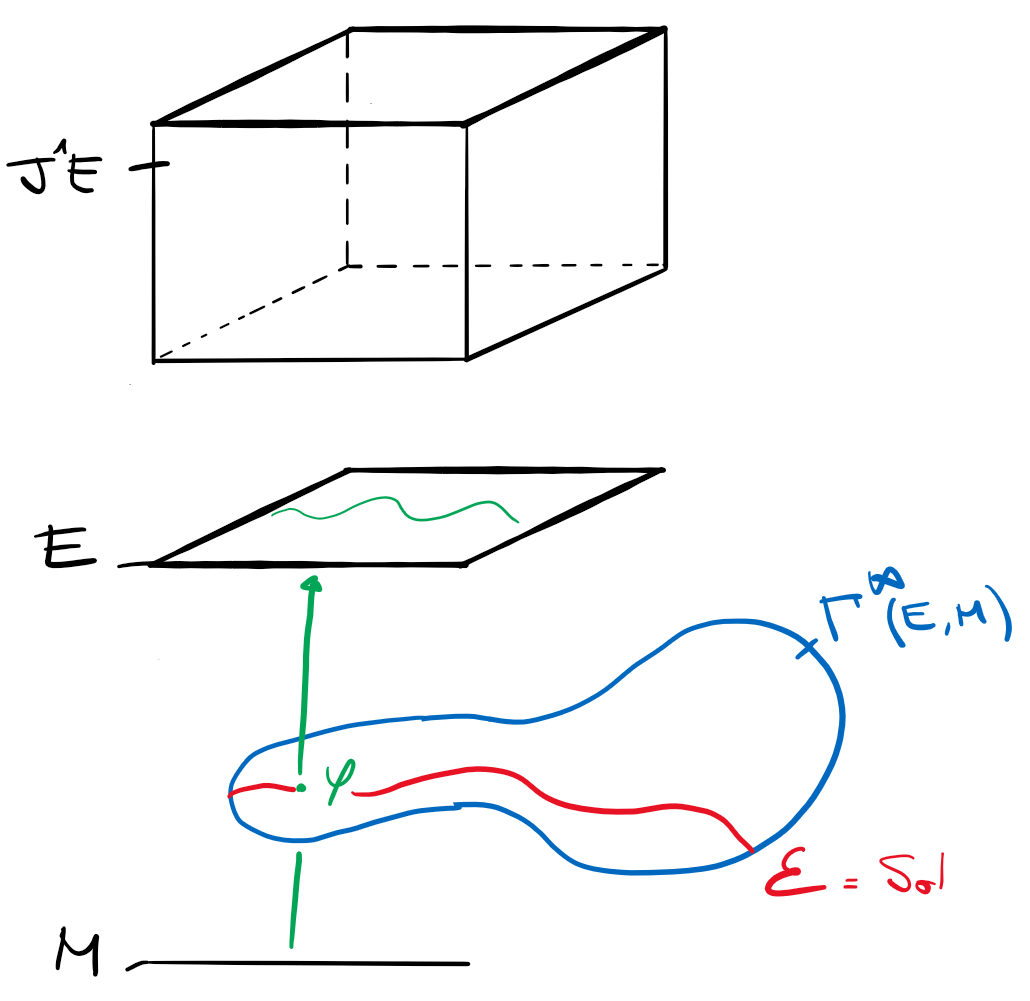
\includegraphics[width=0.9\linewidth]{../Pictures/Covariant}			
			\end{center}
		\end{column}
		%
		\begin{column}{.50\linewidth}
			\begin{itemize}
				\item[•] Consider a classical field $E\to M$ with I-order Lagrangian $\mathcal{L}$;
				\item[•]<2-> $\mathcal{L}$ determines  
					\begin{itemize}
						\item[(a)] a multisymplectic structure on $J^1 E$,
						\item[(b)] a symplectic \emph{Diffiety} $(\mathcal{E})$ called \emph{Covariant phase space}\footnote{Suppose E-L operator being \emph{formally integrable}};
					\end{itemize}
				\item[•]<3-> two different candidates for the role of \emph{physical observables}:
					\begin{itemize}
						\item[(a)] Lie infinity algebra $L_\infty (M,\omega)$;
						\item[(b)] Cochain complex $\bar{\Omega}^\bullet(\mathcal{E})$.
					\end{itemize}																
			\end{itemize}
		\end{column}
		%
	\end{columns}
	%
	\vfill
	%
	\begin{probox}[colbacktitle=yellow!15!white ,colback=yellow!15!white]{ How to mechanically interpret the previous notion of multisym. observables?}
		\begin{itemize}
			\item[\smark] Application to \emph{Multisymplectic PDEs}?
			\item[\smark] Third actor: the \emph{Space of initial datas}.
			\item[\smark] Compatibility of moment maps wrt. lifts of a group action $G \curvearrowright M$ on the base manifold to $J^\infty E$ and the field configuration space $\Gamma(E)$.
			\item[\smark] Is it possible to the latter setting the geometric \cite{Blacker2020} and algebraic \cite{Blacker2022} reduction procedures in terms of the so-called \emph{homotopy zero-locus} \cite{Bernardy2022}?
		\end{itemize}
	\end{probox}			
	
\end{frame}
\note[itemize]{
	\item the two framework yields different candidates to the role of \emph{physical observable}:
	\item Note that in the classical ordinary case the space of initial data coincides with the phase space

}
%-------------------------------------------------------------------------------------------------------------------------------------------------



%-------------------------------------------------------------------------------------------------------------------------------------------------
\begin{frame}{Reduction commutes with Prequantization}

\end{frame}
\note[itemize]{
	\item  Research Line B

}
%-------------------------------------------------------------------------------------------------------------------------------------------------

%-------------------------------------------------------------------------------------------------------------------------------------------------
\begin{frame}{Multisymplectic PDEs and Integrators}

\end{frame}
\note[itemize]{
	\item  Research Line C

}
%-------------------------------------------------------------------------------------------------------------------------------------------------




%---------------------------------------------------------------------------------------------------------------------------------------------------
\begin{frame}{Research proposal context: (multi)symplectic reduction}
	\textbf{\color{UniGreen}Symplectic reduction:}~~
	Procedure associating to any (suitably regular) pair of symplectic manifold and Hamiltonian action another symplectic manifold of smaller dimension.
	\vfill
	\pause
	\begin{thmblock}[Marsden-Weinstein reduction]
		\vspace{-.4em}
		\begin{tabular}{l p{12cm}}
		    Given: & $(M,\omega)$ symplectic
		    \\
		    & $G\curvearrowright M$ symplectic with equivariant momap. $J:M\to \mathfrak{g}^*$
		    \\[.2em]
		    Assume: & $\mu \in \mathfrak{g}^*$ regular value of $J$ 
		    \qquad\quad \footnotesize \textcolor{gray}{($\Rightarrow$ $J^{-1}(\mu)\hookrightarrow M$ smooth embedding)}
		    \\
			& $G_\mu\action J^{-1}(\mu)$ free and proper
			\quad \footnotesize \textcolor{gray}{($\Rightarrow$ $J^{-1}(\mu)/G_\mu$ smooth manifold)}
			\\[.4em]
			Then: & $\exists!$ symplectic structure $\omega_\mu$ in $M_\mu:= J^{-1}(\mu)/G_\mu$ \\
			& s.t. $\pi^\ast \omega_\mu = j^\ast \omega$ with $j:M_\mu \hookrightarrow M$ and $\pi:M\twoheadrightarrow M_\mu$
		\end{tabular}
		\vspace{-.4em}
	\end{thmblock}
	%
	\vfill
	\pause
	\begin{columns}
		\begin{column}{0.40\textwidth}
			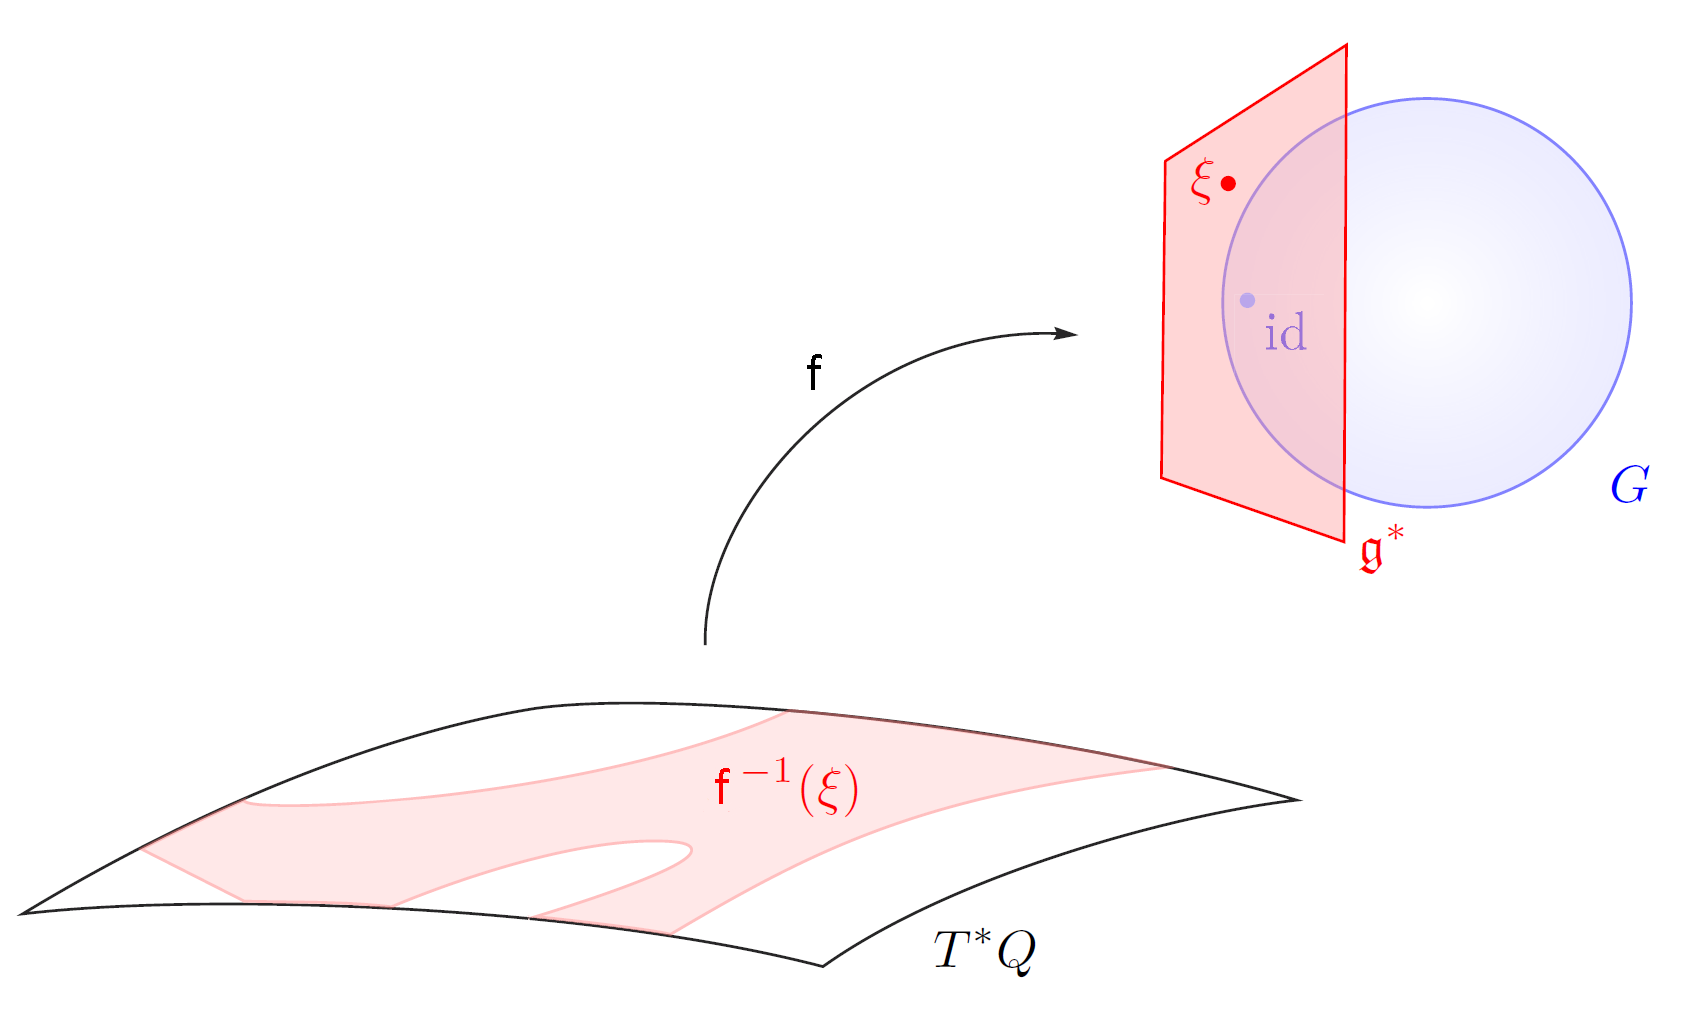
\includegraphics[width=\textwidth]{./Pictures/Reduction}
		\end{column}	
		
		\begin{column}{0.6\textwidth}
				\textbf{\color{UniGreen}In mechanics:}~~
			it embodies the process of restricting the dynamics of the system to the level sets of the conserved quantities pertaining to the symmetry group.		
			\\
			\color{gray}\small( e.g. restricting to studying a point-like particle in a central potential by studying it in radial coordinates only)
		\end{column}	
	\end{columns}	


<\end{frame}
%---------------------------------------------------------------------------------------------------------------------------------------------------


%---------------------------------------------------------------------------------------------------------------------------------------------------
\begin{frame}{Research goals (2022-2023)}
  	%
	\begin{probox}[colback=white]{Multisymplectic regular reduction}
		\begin{itemize}
			\item[\cmark] Recent definition by Blacker:
			\item[\smark] it involves a different notion of \emph{observables};
			\item[\smark] reconcile with the $L_\infty$/homotopy framework.
		\end{itemize}
	\end{probox}
	
	\pause
	\begin{probox}[]{Multisymplectic singular reduction}
		\begin{itemize}
			\item[\cmark] On-going collaboration with Blacker and Ryvkin:
			\item[\smark] complete comparison with other known reduction schemes;
			\item[\smark] higher analogue of \emph{cotangent reduction} theorems;
			\item[\smark] relevant examples.
		\end{itemize}
	\end{probox}

 	\pause
	\begin{probox}[colback=white]{Geometric mechanics perspective}
		\begin{itemize}
			\item[\cmark] MS. geometry stemmed from a geometric formulation of classical field theories:
			\item[\smark] modern development yet to be %fruitfully
			reconciled with physics;
			\item[\smark] reduction of scalar field w.r.t. Poincarè yields the usual field momenta?
			\item[\smark] Streamlined procedure to retrieve ordinary field observables from the multisym. framework.
		\end{itemize}
	\end{probox}  

	\pause
	\begin{probox}[colbacktitle=yellow!15!white ,colback=yellow!15!white]{{[Reduction, Quantization]=0} ?}
		\begin{itemize}
			\item[\cmark] Preliminary results on $2$-plectic prequantization due to Sevestre and Wurzbacher:
			\item[\smark] Investigate compatibility of reduction and prequantization schemes in the multisym. framework.
		\end{itemize}
	\end{probox}	
\end{frame}
%---------------------------------------------------------------------------------------------------------------------------------------------------


%------------------------------------------------------------------------------------------------
% Thank you! slide
%-------------------------------------------------------------------------------------------------------------------------------------------------
	\begin{frame}{}
		\vfill
	  \centering 
	  {\Huge\color{red} 
	  \emph{Thank you for your attention!}}
		\vfill
		%
		\centering
		\begin{columns}
			\hfill
			\begin{column}{0.05\linewidth}
				\centering \includegraphics{beamericonarticle}
			\end{column}
			\begin{column}{0.8\linewidth}
				\centering
				\textbf{On some (multi)symplectic aspects of link invariants},
				\\
				\emph{AMM, Mauro Spera}, \href{https://arXiv.org/abs/1805.01696}{arxiv:1805.01696};\\
				(To appear in \emph{Journal of the Australian Mathematical Society})	
			\end{column}
			\begin{column}{0.05\linewidth}
				\centering \includegraphics{beamericonarticle}			
			\end{column}
			\hfill
		\end{columns}
		\vfill
		\begin{columns}
			\hfill
			\begin{column}{0.05\linewidth}
				\centering \includegraphics{beamericonarticle}
			\end{column}
			\begin{column}{0.8\linewidth}
				\centering
		\textbf{Derivation of the HOMFLYPT knot polynomial via helicity and geometric quantization},
				\\
		\emph{AMM, Mauro Spera}, \href{https://arxiv.org/abs/1910.13400}{arXiv:1910.13400};\\
				(To appear in \emph{Bollettino dell'Unione Matematica Italiana})	
			\end{column}				
			\begin{column}{0.05\linewidth}
				\centering \includegraphics{beamericonarticle}			
			\end{column}
			\hfill
		\end{columns}
		\vfill
		\begin{columns}
			\hfill
			\begin{column}{0.05\linewidth}
				\centering \includegraphics{beamericonarticle}
			\end{column}
			\begin{column}{0.8\linewidth}
				\centering
				\textbf{Observables of multisymplectic manifolds and higher Courant algebroids},
				\\
				\emph{AMM, Marco Zambon};% \href{https://arXiv.org/abs/1805.01696}{arxiv:1805.01696};\\
				(To appear soon on \emph{arxiv})	
			\end{column}
			\begin{column}{0.05\linewidth}
				\centering \includegraphics{beamericonarticle}			
			\end{column}
			\hfill
		\end{columns}
	\end{frame}
%-------------------------------------------------------------------------------------------------------------------------------------------------


%------------------------------------------------------------------------------------------------
% APPENDIX
%------------------------------------------------------------------------------------------------
\appendix
\section{EXTRA}
%\sectionpage
\begin{frame}
	\begin{center}
	\Huge\emph{Backup Slides}
	\end{center}
\end{frame}
\addtocounter{framenumber}{-1}
%------------------------------------------------------------------------------------------------



%-------------------------------------------------------------------------------------------------------------------------------------------------
\begin{frame}[fragile]{Lie $\infty$-algebra of Observables (higher observables) }
	Let be $(M,\omega)$ a $n$-plectic manifold.
	  	\vfill
	\begin{defblock}[$L_\infty$-algebra of observables ~\emph{(Rogers)} \cite{Rogers2010}]
		\medskip
		\hspace{.25em} Is a cochain-complex $(L,\{\cdot\}_1)$ \\
		\vspace{-1em}
		\begin{center}
			\includestandalone{./Pictures/Frame_Observables}
		\end{center}
		\onslide<2->{
			\bigskip
			\hspace{.25em} with $n$ (skew-symmetric) multibrackets $(2 \leq k \leq n+1)$\\
			\vspace{-1em}
			\onslide<3->{
				\begin{center}
					\includestandalone{./Pictures/Equation_Multibracket}	
				\end{center}
			}
			\medskip
		}
		%
	\end{defblock}
  \end{frame}
%-------------------------------------------------------------------------------------------------------------------------------------------------


%-------------------------------------------------------------------------------------------------------------------------------------------------
\begin{frame}[fragile]{Homotopy comomentum maps}
	Consider a Lie algebra action $v:\mathfrak{g} \to \mathfrak{X}(M)$  \underline{preserving the $n$-plectic form $\omega$}.
	\vfill
	\begin{defblock}[Homotopy comomentum map \emph{(Callies, Fregier, Rogers, Zambon)} \cite{Callies2016}]
			\includestandalone{./Pictures/Frame_Lifting}
	\end{defblock}
	\onslide<4->{
	\begin{lemblock}[HCMM unfolded  \cite{Callies2016}]
			%
			HCMM is a sequence of (graded-skew) multilinear maps:
			\begin{displaymath}
				(f)  = \big\lbrace f_k: \; \Lambda^k{\mathfrak g} \to L^{1-k} \subseteq \Omega^{n-k}(M) 
				~\big\vert~ 0\leq k \leq n+1  \big\rbrace
			\end{displaymath}
			\emph{fulfilling:}%\emph{such that:}
			\begin{itemize}
				\item<5-> $f_0 = 0 $, $f_{n+1} = 0$
				\item<6-> $d f_k (p) = f_{k-1} (
				\tikz[baseline,remember picture]{\node[rounded corners,
                        fill=green!5,draw=green!30,anchor=base]            
            			(target) {$\partial $ };
            	}				
				p)  - (-1)^{\frac{k(k+1)}{2}} \iota(v_p) \omega 
				\qquad\scriptstyle \forall p \in \Lambda^k(\mathfrak{g}),\; \forall k=1,\dots n+1$
			\end{itemize}
		\onslide<7->{
			\tikz[overlay,remember picture]
			{
				\node[rounded corners,
	                 draw=green!30,anchor=base]            
	            	 (base) at ($(current page.east)-(3,3)$) [rotate=-0,align=center] {\footnotesize{\hyperlink{frame:CE-complex}{\emph{Chevalley-Eilenberg boundary op.}}}};
			}	
		\begin{tikzpicture}[overlay,remember picture]
	    	\path[->] (base.west) edge[bend right,green](target.north east);
	    \end{tikzpicture}
	    }
	\end{lemblock}	
	}
	\vfill
\end{frame}
%-------------------------------------------------------------------------------------------------------------------------------------------------



%------------------------------------------------------------------------------------------------
\begin{frame}[fragile]{MS geometry and classical field mechanics}
		Consider a smooth manifold $Y$,
		\begin{columns}
			\hfill
			\begin{column}{.5\linewidth}
				\emph{Multicotangent bundle} $\bigwedge = \bigwedge^n T^\ast Y$\\
				is naturally $n$-plectic
			\end{column}
			\begin{column}{.4\linewidth}
				\[
				\begin{tikzcd}
					\Lambda \ar[d,"\pi"'] & T \Lambda \ar[d,"T \pi"] \ar[l] \\
					Y								& T Y \ar[l]
				\end{tikzcd}	
				\]
			\end{column}
		\end{columns}
	\pause
	\begin{defblock}[Tautological $n$-form]
		$\theta \in \Omega^n(\Lambda)$ such that:
		\begin{displaymath}
		\begin{split}
			\left[ \iota_{u_1 \wedge \ldots \wedge u_n} \theta \right]_\eta 
			&= \iota_{(T \pi)_\ast u_1 \wedge \ldots \wedge (T \pi)_\ast u_n} \eta \\
			&= \iota_{u_1 \wedge \ldots \wedge u_n} \pi^\ast \eta 
			\qquad \qquad \forall \eta \in \Lambda \, , \: \forall u_i \in T_\eta \Lambda 		
		\end{split}
		\end{displaymath}
	\end{defblock}
	\vfill
	\begin{columns}
		\begin{column}{.6\linewidth}
			\begin{defblock}[Tautological (multisymplectic) (n+1)-form]
				$$\omega := d \theta$$
			\end{defblock}
		\end{column}
		\begin{column}{.4\linewidth}
		 	\begin{claimblock}$\omega$ is not degenerate.\end{claimblock}	
		\end{column}
	\end{columns}	
	\pause
	\begin{keywordblock}
		\begin{tabular}{|c|c|c|}
			\hline 
			point-particles mechanics & $\rightsquigarrow$ & classical fields mechanics \\
			%(finite discrete DOF) & & (finite dimensional continuous DOF) \\
			\hline 
			symplectic & $\rightsquigarrow$ & multisymplectic \\ 
			\hline 
			Observables (Poisson) algebra & $\rightsquigarrow$ & Observables $L-\infty$ algebra
			 \\ 
			\hline 
			Co-moment map & $\rightsquigarrow$ & Homotopy co-momentum map \\ 
			\hline 
		\end{tabular} 
	\end{keywordblock}

	
\end{frame}
\note[itemize]{
	\item This example is significant from the perspective of geometric classical field theory:
		\begin{displaymath}
			\frac{\text{classical mechanics}}{\text{symplectic geo.}} =
			\frac{\text{classical field mechanics}}{\text{multisymplectic geo.}}
		\end{displaymath}
	\item Multicotangent bundle is the \emph{Higher analogue} of the cotangent bundle.
	(but it is not yet the analogue of a \emph{phase space}.)
\item The multiphase space is the sub-bundle of $n$-forms vanishing when contracted with 2 vertical fields.
  	\item The reason why this sub-bundle has a particular role is that it can be proved to be isomorphic to a suitable dual of the first Jet bundle.
  	\item For further details see Gotay et al. \href{https://arxiv.org/abs/physics/9801019}{arXiv:physics/9801019}. For a pictorial representation of all the structures involved in the geometric mechanics of I order classical field theories see appendix, pag: \ref{frame:Gimmsy}.
}
%------------------------------------------------------------------------------------------------

%------------------------------------------------------------------------------------------------
  \begin{frame}[fragile]{GIMMSY construction} \label{frame:Gimmsy}
  		\includestandalone[width=0.90\textwidth]{./Pictures/Figure_ms_landscape}  	
  \end{frame}
  \note{}
%------------------------------------------------------------------------------------------------


%-------------------------------------------------------------------------------------------------------------------------------------------------
\subsection{Multisymplectic singular reduction}

%-------------------------------------------------------------------------------------------------------------------------------------------------
\begin{frame}{Singular Reduction: Roadmap}
	%
	\begin{block}{Data:}
			\begin{itemize}
				\item A \emph{constraint set} $N$ (possibly singular),
				\item An infinitesimal action preserving $N$.
			\end{itemize}
	\end{block}
	%
	\vfill
	\pause
	%
	\begin{block}{Goal:}
		\begin{itemize}
			\item Obtain a "reduced" observables algebra out of the data.
		\end{itemize}
	\end{block}
	%
	\vfill
	\pause
	%
	\begin{block}{Strategy:}
		\begin{enumerate}
			\item Define smooth fields/forms \emph{tangent to $N$},
			\item define smooth fields/forms \emph{vanishing along $N$},
			\item define \emph{reducible fields} requiring the preservation of the vanishing objects,
			\item define \emph{reducible forms} requiring their conservation w.r.t. the infinitesimal action,
			\item define \emph{reducible and vanishing observables},
			\item \textbf{quotient}
		\end{enumerate}
	\end{block}






\end{frame}

%-------------------------------------------------------------------------------------------------------------------------------------------------


%-------------------------------------------------------------------------------------------------------------------------------------------------
\begin{frame}[shrink]{Smooth objects on a singular set}
	Consider $N$ closed subset of $M$.
	\vfill
	\pause
	\begin{defblock}
	 $I_N$ = ideal of smooth functions vanishing over $N$.
	\end{defblock}
	\vfill
	\pause

	\begin{columns}[T]
		\setlength{\belowdisplayskip}{5pt}
		\begin{column}{.65\linewidth}
			%
			\centering \it
				\begin{defblock}[v.f tangent to $N$]
					\begin{displaymath}
						\X_N(M):=
						\left\lbrace
							v \in \X(M)
						~\Big\vert~
							\L_v(I_N) \subseteq I_N
						\right\rbrace
					\end{displaymath}
				\end{defblock}
				\begin{defblock}[v.f vanishing on $N$]
					\begin{displaymath}
						I_\X(N):=
						\left\lbrace
							v \in \X(M)
						~\Big\vert~
							\L_v(C^\infty(M)) \subseteq I_N
						\right\rbrace
					\end{displaymath}				
				\end{defblock}				
		\end{column}	
		%
		%
		\begin{column}{.35\linewidth}
			\centering 
			\includestandalone[width=0.8\textwidth]{Pictures/Figure_VfTangentN}			
		\end{column}	
	\end{columns}			
	%	
	\pause

				%

				%	
		\begin{tcolorbox}[
		enhanced,frame hidden,borderline={0.5pt}{0pt}{blue},
		arc=5pt,colback=white,
		colbacktitle=white,]
			\color{blue}{\textbf{Lem}:} If $N$ is smoothly embedded,  $\X(N)\cong {X_N(M)}/{I_\X}$.
		\end{tcolorbox}

		\pause

		\begin{defblock}[Differential form vanishing on $N$]
			\begin{displaymath}
				I_{\Omega(N)}:=
				\left\lbrace
					\alpha\in\Omega^k(M
				~\left\vert~
					\begin{array}{l r}
						k\geq 0,~		\\		
						\alpha(u_1,\ldots,u_k) \in I_N & \forall u_i \in\X_N(M)
					\end{array}
				\right\rbrace\right.
			\end{displaymath}
		\end{defblock}

\end{frame}
\note[itemize]{
 \item $N$ is not a submanifold in general. An example is $N=\mu^{-1}(0)$ for a certain smooth map $N$.
 \item observe that if $N$ is a smooth embedded submanifold, one has that $\X(N)\cong \frac{X_N(M)}{I_\X}$  

}
%-------------------------------------------------------------------------------------------------------------------------------------------------



%-------------------------------------------------------------------------------------------------------------------------------------------------
\begin{frame}{Reducible smooth objects \quad \small (w.r.t. $N$ and $\g\action M$)}
	Consider $\g \action M$ by vector fields tangent to $N$ % \hfill( fond. distribution $\underline{\g}\subseteq \X_N(M)$)
	\\
	\vfill
	Denote by :  
	\hspace{1em} $\underline{\g}\subseteq \X_N(M)$ the fundamental distribution,
	\\
	\hspace{6.5em}  $\X_g$ the $C^\infty$-module generated by $\underline{\g}$.
	\\
	\vfill
	\begin{defblock}[Reducible v.fields ]
			\begin{displaymath}
				\X(M)_{[N]} :=
				\left\lbrace
					v \in \X(M)
				~\left\vert~
					\begin{array}{l}
						\L_v (I_N) \subseteq I_N	\\		
						\L_v (\X_g) \subseteq \X_g + I_\X
					\end{array}
				\right\rbrace\right.
			\end{displaymath}
%			\blfootnote{
%			 $\X_g$ = $C^\infty(M)$-module generated by the fundamental distribution.
%			}	

	\end{defblock}	
	%
	\pause
	%
	\begin{defblock}[Reducible forms ]
		\begin{displaymath}
			\Omega(M)_{[N]} :=
			\left\lbrace
				\alpha \in \Omega(M)
			~\left\vert~
				\begin{array}{l r}
					\L_\underline{\xi} \,\alpha \in I_{\Omega(N)}	\\		
					\iota_\underline{\xi} \,\alpha \in I_{\Omega(N)}	& \forall \xi \in \g				\end{array}
			\right\rbrace\right.
		\end{displaymath}	
	\end{defblock}	
	%
	\pause
	%
	\begin{defblock}[Reducible Hamiltonian forms]
		\begin{displaymath}
			(\Omega(M)_{ham}^{n-1})_{[N]} :=
			\left\lbrace
				\alpha \in \Omega(M)_{ham}^{n-1}
			~\left\vert~
				\begin{array}{l r}
					\alpha \text{ is a reducible form} \\
					\vHam_\alpha \text{ is a reducible v.field}
				\end{array}
			\right\rbrace\right.
		\end{displaymath}	
	\end{defblock}		

	
\end{frame}
\note[itemize]{
 \item $\g\action M$ by vector field tangent to $N$ means that $\underline{\xi}\in\X_n(M) \forall \xi \in \g$
 \item Spelling out the definition: reducible vector fields are 
 \\i) v.f. tangent to N 
 \\ii) such that their commutator with any $\underline{\xi}$ lies in $\X_\g$ along $N$.
 \item more algebraically, they stabilize both $I_N$ and $\X_g + I_\X$.
 \item observe that $\L_v I_\X \subseteq I_\X$ since , $\forall u \in I_\X$ $\forall f \in C^\infty(M)$ one has\\
 $(\L_v u) f = \L_{[v,u]} f = \L_v\L_u f - \L_u\L_v f \in I_N$
 \item
}
%-------------------------------------------------------------------------------------------------------------------------------------------------

%-------------------------------------------------------------------------------------------------------------------------------------------------
\begin{frame}{Singular reduction}
	\begin{defpropblock}[Reducible $L_\infty$-observables]
		Is the {\color{blue!70!black}$L_\infty$-subalgebra} of $L_\infty(M,\omega)$ given by
		\begin{displaymath}
			L_\infty(M,\omega)_{[N]}^k :=
			\begin{cases}
				\Omega^{n-1-k}(M)_{[N]} 
				\qquad\text{\color{gray}\small (reducible forms) }
				& \text{if } n-1\leq k < 0 \\
				(\Omega(M)_{ham}^{n-1})_{[N]} 
				\quad
				\text{\color{gray}\small (reducible hamiltonians) }
				& \text{if } k = 0 \\
				0 & \text{if } k > 0
			\end{cases}
		\end{displaymath}
	\end{defpropblock}
	%
	\pause
	%
	\begin{defpropblock}[Vanishing $L_\infty$-observables]
		Is the {\color{blue!70!black}$L_\infty$-ideal} of $L_\infty(M,\omega)_{[N]}$ given by
		\begin{displaymath}
			I_{L_\infty(M,\omega)} :=
			\left\lbrace
				\alpha \in L_\infty(M,\omega)_{[N]}
			~\left\vert~
				\begin{array}{l l}
					\alpha(v_1,\dots,v_k) \in I_N  \quad \forall v_i \in \X_N &
					\text{if}~ \alpha \in \Omega^k \\
					\vHam_\alpha \in \X_\g + I_\X &
					\text{if}~ \alpha \in \Omega^{n-1}
				\end{array}
			\right\rbrace\right.
		\end{displaymath}
	\end{defpropblock}
	%
	\pause
	%
	\begin{defblock}[Reduced $L_\infty$-algebra of observables]
		Is the $L_\infty$-quotient : \quad
		$\dfrac{L_\infty(M,\omega)_{[N]}^k}{I_{L_\infty(M,\omega)}}$
	\end{defblock}

\end{frame}
\note[itemize]{
 \item The graded vector space underlying the reduced $L_\infty$-algebra $\Ham_\infty(M,\omega)_N$ is explicitly given by
\begin{displaymath}
	\Ham_\infty(M,\omega)_N =
	\frac{
		\left\lbrace
			(\alpha,v) \in \Omega(M){[n{-}1]}\oplus\X(M)
		~\left\vert~
			\begin{array}{l l}
				\iota_v \omega = -\d \alpha^{(0)} &
				\\
				\iota_\xi \alpha \in I_{\Omega}(N) &
				\\
				\L_\xi\alpha \in I_{\Omega}(N)
				&
				\\
				\L_\xi v \in \fgmodule +\vanvf
				&~\forall \xi \in \g 
				\\
				v \in \X_N(M)
				&
			\end{array}
		\right.
		\right\rbrace
	}{
		\left\lbrace
			(\alpha,v) \in \Omega(M){[n{-}1]}\oplus\X(M)
		~\left\vert~
			\begin{array}{l}
				\alpha \in I_{\Omega}(N)
				\\
				v \in \fgmodule +\vanvf
			\end{array}
		\right.
		\right\rbrace
	}~.
\end{displaymath}
}
%-------------------------------------------------------------------------------------------------------------------------------------------------

%-------------------------------------------------------------------------------------------------------------------------------------------------
\begin{frame}{Singular reduction (Upshot and conclusions)}

	\begin{itemize}
		\item Consider $N=\mu^{-1}(0)$ to be regular (smooth embedding)
		\vspace{.5em}
		\begin{table}[]
			\begin{tabular}{ccc}
			Multisymplectic               &                      & Multisymplectic                  \\
			regular                       & $\equiv$             & singular                \\
			reduction & & reduction
			\end{tabular}
		\end{table}	
		
		\pause
		\item
			Consider $\omega$ to be $1$-plectic
			\vspace{.5em}
			\begin{table}[]
				\begin{tabular}{ccc}
				Multisymplectic               &                      &  Sniaticky--Weinstein                  \\
				singular                       & $\cancel\equiv$             & singular                \\
				reduction & & reduction
				\end{tabular}
			\end{table}	

			(but $\exists$ a canonical Poisson algebra morphism)
	\end{itemize}
	
	\pause
			\vfill
		  \centering 
		  {\Huge\color{red} 
		  \emph{Thank you for your attention!}}
			\vfill
\end{frame}
\note[itemize]{
 \item
}
%-------------------------------------------------------------------------------------------------------------------------------------------------


%------------------------------------------------------------------------------------------------
\begin{frame}\frametitle{Reduction of states vs.\ reduction of observables}
	\begin{minipage}{\textwidth}
	\hspace{-.4cm}
	\begin{tikzpicture}
		\draw (-4,-2.5) rectangle (4,2.5);
		\draw (-4,0) -- (4,0);
		\draw (0,-2.5) -- (0,2.5);

		\draw node[align=center] at (-2,1.25) {symplectic\\ reduction};
		\draw node[align=center] at (2,1.25) {multisymplectic\\ reduction};
		\draw node[align=center] at (-2,-1.25) {\'{S}niatycki--Weinstein,\\Dirac,\\Arms--Gotay--Jennings\\ reduction};
		\draw node[align=center] at (2,-1.25) {\color{UniGreen}$L_\infty$ reduction};

		\draw node[align=center] at (2,2.85) {\color{UniGreen}\emph{higher}};
		\draw node[align=center] at (-2,2.85) {\emph{lower}};

		\draw node[align=right] at (-4.7,1.25) {\emph{states}};
		\draw node[align=right] at (-5.13,-1.25) {\color{UniGreen}\emph{observables}};
	\end{tikzpicture}
	\end{minipage}
\end{frame}
%------------------------------------------------------------------------------------------------

%------------------------------------------------------------------------------------------------
\begin{frame}\frametitle{Auxiliary constructions}
	\begin{minipage}{\textwidth}
	\centering
	\scalebox{.65}{
	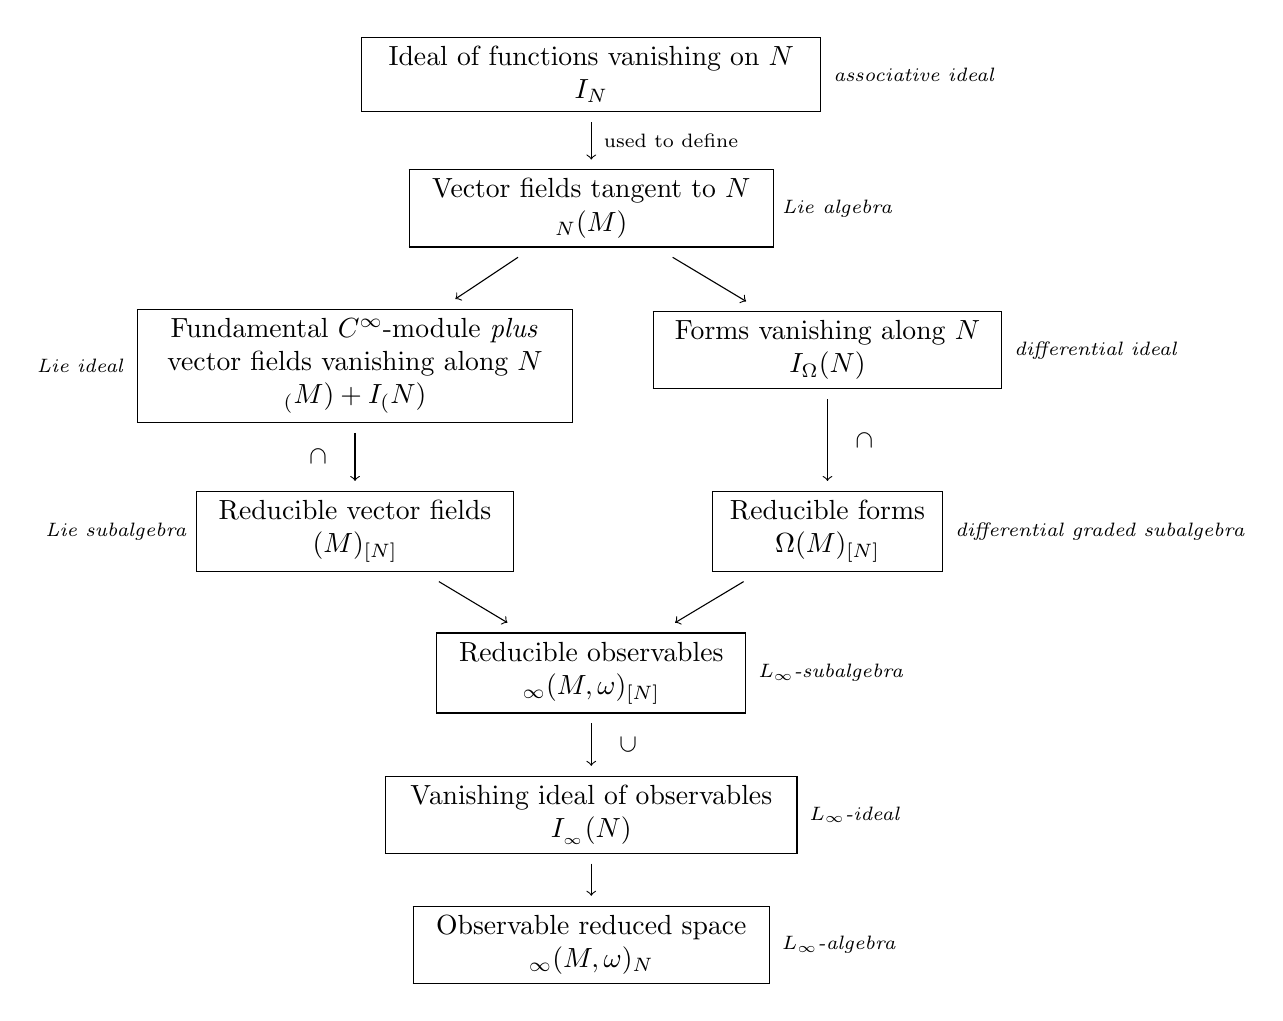
\begin{tikzpicture}
		\node (A) at (0,10.0) {\fbox{\parbox{5.6cm}{\centering Ideal of functions vanishing on $N$ \\ $I_N$}}};
		\node (B) at (0,8.3) {\fbox{\parbox{4.4cm}{\centering Vector fields tangent to $N$ \\ $\X_N(M)$}}};
		\node (C) at (3,6.5) {\fbox{\parbox{4.2cm}{\centering Forms vanishing along $N$ \\ $I_\Omega(N)$}}};
		\node (D) at (3,4.2) {\fbox{\parbox{2.7cm}{\centering Reducible forms \\ $\Omega(M)_{[N]}$}}};
		\node (E) at (-3,6.3) {\fbox{\parbox{5.3cm}{\centering Fundamental $C^\infty$-module \emph{plus} \\ vector fields vanishing along $N$ \\ $\X_\g(M)+I_\X(N)$}}};
		\node (E') at (-3,4.2) {\fbox{\parbox{3.8cm}{\centering Reducible vector fields \\ $\X(M)_{[N]}$}}};
		\node (F) at (0,2.4) {\fbox{\parbox{3.7cm}{\centering Reducible observables \\ $\Ham_\infty(M,\omega)_{[N]}$}}};
		\node (G) at (0,0.6) {\fbox{\parbox{5.0cm}{\centering Vanishing ideal of observables \\ $I_{\Ham_\infty}(N)$}}};
		\node (H) at (0,-1.05) {\fbox{\parbox{4.3cm}{\centering Observable reduced space \\ $\Ham_\infty(M,\omega)_N$}}};

		\draw[->] (A)-- node[right=1pt]{{\scriptsize used to define}} (B);
		\draw[->] (B)-- (C);
		\draw[->] (C)-- node[right=.25cm]{\rotatebox{-90}{\small $\subset$}} (D);
		\draw[->] (B)-- (E);
		\draw[->] (D)-- (F);
		\draw[->] (E)-- node[left=.25cm]{\rotatebox{-90}{\small $\subset$}} (E');
		\draw[->] (E')-- (F);
		\draw[->] (F)-- node[right=.25cm]{\rotatebox{90}{\small $\subset$}} (G);
		\draw[->] (G)-- (H);

		\node[right=2.95cm] at (A) {\scriptsize\emph{associative ideal}};
		\node[right=2.30cm] at (B) {\scriptsize\emph{Lie algebra}};
		\node[right=2.25cm] at (C) {\scriptsize\emph{differential ideal}};
		\node[right=1.5cm] at (D) {\scriptsize\emph{differential graded subalgebra}};
		\node[left=2cm] at (E') {\scriptsize\emph{Lie subalgebra}};
		\node[left=2.8cm] at (E) {\scriptsize\emph{Lie ideal}};
		\node[right=2cm] at (F) {\scriptsize\emph{$L_\infty$-subalgebra}};
		\node[right=2.65cm] at (G) {\scriptsize\emph{$L_\infty$-ideal}};
		\node[right=2.3cm] at (H) {\scriptsize\emph{$L_\infty$-algebra}};
	\end{tikzpicture}
	}
	\end{minipage}
\end{frame}
%------------------------------------------------------------------------------------------------

%------------------------------------------------------------------------------------------------
\begin{frame}\frametitle{Comparison with geometric reduction}

	Let $(M_N,\omega_N)$ be the geometric reduction of $\g\curvearrowright(M,\omega)$ along $N$.

	\vspace{5pt}
	\begin{theorem}[B.--Miti--Ryvkin]
		The geometric reduction map
		\begin{align*}
			r_N:	\Ham_\infty(M,\omega)_{[N]}	&\to		\Ham_\infty(M_N,\omega_N)		\\
			(v,\alpha)\;			&\mapsto	\;(v_N,\alpha_N)			\\
			\alpha\;			&\mapsto	\;\alpha_N
		\end{align*}
		is a strict $L_\infty$-morphism with kernel $I_{\Ham_\infty}(N)$. In particular, there is a natural inclusion of $L_\infty$-algebras
		\[
		\Ham_\infty(M,\omega)_N = \frac{\Ham_\infty(M,\omega)_{[N]}}{I_{\Ham_\infty}(N)} \;\xhookrightarrow{\;\bar{r}_N\;}\; \Ham_\infty(M_N,\omega_N).
		\]
	\end{theorem}
\end{frame}
%------------------------------------------------------------------------------------------------




%------------------------------------------------------------------------------------------------
% https://en.wikibooks.org/wiki/LaTeX/Bibliographies_with_biblatex_and_biber
\begin{frame}[t,allowframebreaks]{Extended Bibliography}
	\bibliographystyle{alpha}
	\bibliography{bibfile}
\end{frame}
%------------------------------------------------------------------------------------------------




%----------------------------------------------------------------------------------------------------------------------------------
\end{document}
%----------------------------------------------------------------------------------------------------------------------------------
%-------------------------------------------------------------------------------------------------------------------------------------------------




